%==============================================================
% MEMORIA PRÁCTICA 1 - TAR (Técnicas Avanzadas de Robótica)
% ROS 2 Humble
%==============================================================
\documentclass[12pt, a4paper]{report}

%--- Paquetes ---
\usepackage[utf8]{inputenc}
\usepackage[T1]{fontenc}
\usepackage[spanish]{babel}
\usepackage{geometry}
\usepackage{graphicx}
\usepackage{float}
\usepackage{hyperref}
\usepackage{listings}
\usepackage{xcolor}
\usepackage{fancyhdr}
\usepackage{titlesec}
\usepackage{enumitem}
\usepackage{amsmath}
\usepackage{booktabs}
\usepackage{caption}
\usepackage{subcaption}
\usepackage{parskip}

%--- Geometría de página ---
\geometry{
  top=2.5cm,
  bottom=2.5cm,
  left=3cm,
  right=2.5cm
}

\setlength{\headheight}{14pt}

%--- Colores ---
\definecolor{azulROS}{RGB}{0, 100, 180}
\definecolor{grisClaro}{RGB}{245, 245, 245}
\definecolor{verdeCode}{RGB}{0, 128, 0}
\definecolor{rojoComentario}{RGB}{150, 0, 0}

%--- Estilo de código ---
\lstdefinestyle{bash}{
  backgroundcolor=\color{grisClaro},
  basicstyle=\ttfamily\small,
  breaklines=true,
  frame=single,
  framerule=0.5pt,
  rulecolor=\color{azulROS},
  keywordstyle=\color{azulROS}\bfseries,
  commentstyle=\color{rojoComentario}\itshape,
  stringstyle=\color{verdeCode},
  showstringspaces=false,
  tabsize=2,
  captionpos=b,
  numbers=left,
  numberstyle=\tiny\color{gray},
  numbersep=5pt
}

\lstdefinestyle{python}{
  language=Python,
  backgroundcolor=\color{grisClaro},
  basicstyle=\ttfamily\small,
  breaklines=true,
  frame=single,
  framerule=0.5pt,
  rulecolor=\color{azulROS},
  keywordstyle=\color{azulROS}\bfseries,
  commentstyle=\color{rojoComentario}\itshape,
  stringstyle=\color{verdeCode},
  showstringspaces=false,
  tabsize=2,
  captionpos=b,
  numbers=left,
  numberstyle=\tiny\color{gray},
  numbersep=5pt
}

\lstset{
  style=bash,
  extendedchars=true,
  literate=
    {á}{{\'{a}}}1 {é}{{\'{e}}}1 {í}{{\'{i}}}1 {ó}{{\'{o}}}1 {ú}{{\'{u}}}1
    {Á}{{\'{A}}}1 {É}{{\'{E}}}1 {Í}{{\'{I}}}1 {Ó}{{\'{O}}}1 {Ú}{{\'{U}}}1
    {ñ}{{\~{n}}}1 {Ñ}{{\~{N}}}1
    {¿}{{?`}}1   {¡}{{!`}}1
}

%--- Cabecera y pie de página ---
\pagestyle{fancy}
\fancyhf{}
\fancyhead[L]{\small TAR -- Práctica 1: Aprendiendo las bases de ROS 2}
\fancyhead[R]{\small \textit{Apellido Apellido, Nombre}}
\fancyfoot[C]{\thepage}
\renewcommand{\headrulewidth}{0.4pt}

%--- Formato de títulos ---
\titleformat{\chapter}[block]
  {\normalfont\Large\bfseries\color{azulROS}}
  {\thechapter.}{1em}{}
\titleformat{\section}[block]
  {\normalfont\large\bfseries}
  {\thesection}{1em}{}
\titleformat{\subsection}[block]
  {\normalfont\normalsize\bfseries}
  {\thesubsection}{1em}{}

%--- Hiperlinks ---
\hypersetup{
  colorlinks=true,
  linkcolor=azulROS,
  urlcolor=azulROS,
  citecolor=azulROS,
  pdftitle={Práctica 1 TAR - ROS 2 Humble},
  pdfauthor={Apellido Apellido, Nombre}
}

%==============================================================
\begin{document}
%==============================================================

%==============================================================
% PORTADA
%==============================================================
\begin{titlepage}
  \centering

  \vspace*{1cm}

  {\Large \textsc{Universidad de Alicante}}\\[0.3cm]
  {\large \textsc{Escuela Politécnica Superior}}\\[0.5cm]
  \rule{\linewidth}{0.4pt}\\[0.4cm]

  {\large Técnicas Avanzadas de Robótica (TAR)}\\[1.5cm]

  {\Huge \bfseries \color{azulROS} Práctica 1}\\[0.5cm]
  {\LARGE  Bases de ROS 2 (Humble)}\\[2cm]

  \rule{\linewidth}{0.4pt}\\[0.8cm]

  \begin{minipage}{0.45\textwidth}
    \begin{flushleft}
      \textbf{Autor:}
     	Hernández Delgado, Jaime
    \end{flushleft}
  \end{minipage}
  \hfill
  \begin{minipage}{0.45\textwidth}
    \begin{flushright}
      \textbf{Curso:} 2025--2026\\
    \end{flushright}
  \end{minipage}

  \vspace{1.5cm}
  \rule{\linewidth}{0.4pt}

  \vfill

  \textbf{Repositorio GitHub:}\\
  \url{https://github.com/nickhernd/TAR}

  \vspace{1cm}
  {\large \today}

\end{titlepage}

\newpage


\tableofcontents
\newpage

%==============================================================
% PARTE 1: PRIMEROS PASOS
%==============================================================
\chapter{Parte 1: Primeros Pasos}

%--------------------------------------------------------------
\section{Creación del espacio de trabajo}
%--------------------------------------------------------------

En esta sección se describe el proceso de creación y configuración del espacio de trabajo ROS 2 (\texttt{ros2\_ws}), así como la instalación del entorno Docker con ROS 2 Humble.

% Describe brevemente los pasos realizados y añade capturas si lo crees necesario.

%--------------------------------------------------------------
\section{Ejemplo de un entorno: Nodos y Topics}
%--------------------------------------------------------------

\subsection*{Pregunta 1}
\textit{¿Qué podemos saber de este nodo? (Suscriptores, topics)}

\textbf{Respuesta:}\\
% Escribe tu respuesta aquí.

% Si tienes captura, inclúyela así:
% \begin{figure}[H]
%   \centering
%   \includegraphics[width=0.85\textwidth]{parte1/imagenes/p1_nodo_info.png}
%   \caption{Información del nodo \texttt{/talker} con \texttt{ros2 node info}.}
%   \label{fig:p1_nodo_info}
% \end{figure}

\subsection*{Pregunta 2}
\textit{¿Qué podemos saber sobre el topic que publica el nodo que acabamos de lanzar?}

\textbf{Respuesta:}\\
% Escribe tu respuesta aquí.

% \begin{figure}[H]
%   \centering
%   \includegraphics[width=0.85\textwidth]{parte1/imagenes/p1_topic_info.png}
%   \caption{Información del topic \texttt{/chatter}.}
%   \label{fig:p1_topic_info}
% \end{figure}

\subsection*{Pregunta 3}
\textit{¿Qué podemos saber sobre el nuevo nodo \texttt{/listener}?}

\textbf{Respuesta:}\\
% Escribe tu respuesta aquí.

% \begin{figure}[H]
%   \centering
%   \includegraphics[width=0.85\textwidth]{parte1/imagenes/p1_listener_info.png}
%   \caption{Información del nodo \texttt{/listener}.}
%   \label{fig:p1_listener_info}
% \end{figure}

\subsection*{Pregunta 4}
\textit{¿Qué ha sucedido ahora en el topic \texttt{/chatter}?}

\textbf{Respuesta:}\\
% Escribe tu respuesta aquí.

% \begin{figure}[H]
%   \centering
%   \includegraphics[width=0.85\textwidth]{parte1/imagenes/p1_chatter_subs.png}
%   \caption{Estado del topic \texttt{/chatter} tras conectar el listener.}
%   \label{fig:p1_chatter_subs}
% \end{figure}

\subsection*{Pregunta 5}
\textit{¿Qué podemos saber a partir del gráfico de \texttt{rqt\_graph}?}

\textbf{Respuesta:}\\
% Escribe tu respuesta aquí.

\begin{figure}[H]
  \centering
  % \includegraphics[width=0.85\textwidth]{parte1/imagenes/p1_rqt_graph.png}
  \fbox{\parbox{0.8\textwidth}{\centering\vspace{2cm} [Captura rqt\_graph] \vspace{2cm}}}
  \caption{Gráfico \texttt{rqt\_graph} con los nodos \texttt{/talker} y \texttt{/listener}.}
  \label{fig:p1_rqt_graph}
\end{figure}

%--------------------------------------------------------------
\section{Servicios}
%--------------------------------------------------------------

\subsection*{Pregunta 6}
\textit{¿Qué puedes comentar acerca de este servicio?}

\textbf{Respuesta:}\\
% Escribe tu respuesta aquí.

% \begin{figure}[H]
%   \centering
%   \includegraphics[width=0.85\textwidth]{parte1/imagenes/p1_servicio_suma.png}
%   \caption{Ejecución del servicio de suma.}
%   \label{fig:p1_servicio_suma}
% \end{figure}

\subsection*{Pregunta 7}
\textit{Al lanzar el servidor y ejecutar \texttt{ros2 service list} ¿Qué servicios aparecen? ¿Cómo se ha creado el servicio \texttt{minimal\_service} y cuál es su cometido?}

\textbf{Respuesta:}\\
% Escribe tu respuesta aquí.

% \begin{figure}[H]
%   \centering
%   \includegraphics[width=0.85\textwidth]{parte1/imagenes/p1_service_list.png}
%   \caption{Listado de servicios con \texttt{ros2 service list}.}
%   \label{fig:p1_service_list}
% \end{figure}

\subsection*{Pregunta 8}
\textit{¿Cómo puedo saber cuáles son los parámetros de la ``petición'' y de la ``respuesta'' de un servicio? ¿De qué tipología son estos parámetros?}

\textbf{Respuesta:}\\
% Escribe tu respuesta aquí. Ejemplo de comando:
\begin{lstlisting}[style=bash, caption={Mostrar interfaz del servicio con ros2 interface show.}]
ros2 interface show <tipo_servicio>
\end{lstlisting}

% \begin{figure}[H]
%   \centering
%   \includegraphics[width=0.85\textwidth]{parte1/imagenes/p1_interface_show.png}
%   \caption{Salida de \texttt{ros2 interface show} para el servicio de suma.}
%   \label{fig:p1_interface_show}
% \end{figure}

%--------------------------------------------------------------
\section{Ejercicios}
%--------------------------------------------------------------

\subsection{Ejercicio 1: Publicar mensaje al topic \texttt{/chatter}}

\textit{Publica desde la terminal un mensaje al topic \texttt{/chatter} para que sea leído por el nodo \texttt{/listener}.}

\textbf{Comandos utilizados:}
\begin{lstlisting}[style=bash, caption={Publicación manual en el topic /chatter.}]
ros2 topic pub /chatter std_msgs/msg/String "data: 'Tu mensaje aquí'"
\end{lstlisting}

% \begin{figure}[H]
%   \centering
%   \includegraphics[width=0.85\textwidth]{parte1/imagenes/p1_ej1_pub.png}
%   \caption{Publicación de mensaje en \texttt{/chatter} y recepción en \texttt{/listener}.}
%   \label{fig:p1_ej1_pub}
% \end{figure}

\subsection{Ejercicio 2: Modificar el servicio suma}

\textit{Cambia el servicio \texttt{servicio\_suma} para que calcule: \(a + b - c \cdot d \div e\), siendo \(a, b, c, d, e\) valores enteros (\texttt{int64}) y el resultado en \texttt{float64}.}

\textbf{Descripción de los cambios:}\\
% Explica qué archivos has modificado y cómo.

\textbf{Archivos modificados:}
\begin{itemize}
  \item \texttt{interfaz\_servicio\_suma/srv/...} -- Modificación de la interfaz del servicio.
  \item \texttt{servicio\_suma/...} -- Modificación del servidor y cliente.
\end{itemize}

% \begin{figure}[H]
%   \centering
%   \includegraphics[width=0.85\textwidth]{parte1/imagenes/p1_ej2_resultado.png}
%   \caption{Resultado de la ejecución del servicio modificado.}
%   \label{fig:p1_ej2_resultado}
% \end{figure}

%==============================================================
% PARTE 2: NIVEL PRINCIPIANTE
%==============================================================
\chapter{Parte 2: Nivel Principiante}

%--------------------------------------------------------------
\section{Crear un Paquete}
%--------------------------------------------------------------

\subsection*{Pregunta 9}
\textit{¿Qué comando me indica todas las dependencias que puedo usar en mis paquetes?}

\textbf{Respuesta:}\\
% Escribe tu respuesta aquí.

\begin{lstlisting}[style=bash, caption={Comando para listar dependencias disponibles.}]
% Escribe aquí el comando
\end{lstlisting}

%--------------------------------------------------------------
\section{Crear un Mensaje}
%--------------------------------------------------------------

\subsection*{Pregunta 10}
\textit{¿Qué comando se debe utilizar para saber de qué tipo es el mensaje creado?}

\textbf{Respuesta:}\\
% Escribe tu respuesta aquí.

\begin{lstlisting}[style=bash, caption={Comando para verificar el tipo de mensaje MiMensaje.}]
% Escribe aquí el comando
\end{lstlisting}

% \begin{figure}[H]
%   \centering
%   \includegraphics[width=0.85\textwidth]{parte2/imagenes/p2_msg_type.png}
%   \caption{Verificación del tipo de mensaje \texttt{MiMensaje}.}
%   \label{fig:p2_msg_type}
% \end{figure}

\subsection*{Pregunta 11}
\textit{Muestra el gráfico de entorno ROS generado usando \texttt{rqt\_graph}.}

\begin{figure}[H]
  \centering
  % \includegraphics[width=0.85\textwidth]{parte2/imagenes/p2_rqt_graph.png}
  \fbox{\parbox{0.8\textwidth}{\centering\vspace{2cm} [Captura rqt\_graph Parte 2] \vspace{2cm}}}
  \caption{Gráfico \texttt{rqt\_graph} con los nodos \texttt{nodo\_envia} y \texttt{nodo\_recibe}.}
  \label{fig:p2_rqt_graph}
\end{figure}

\subsection*{Pregunta 12}
\textit{Intenta modificar la constante nombre del mensaje, modificando el código de \texttt{nodo\_envia}. ¿Qué sucede?}

\textbf{Respuesta:}\\
% Escribe tu respuesta aquí. Explica el error o comportamiento observado.

% \begin{figure}[H]
%   \centering
%   \includegraphics[width=0.85\textwidth]{parte2/imagenes/p2_const_error.png}
%   \caption{Error al intentar modificar la constante \texttt{NOMBRE}.}
%   \label{fig:p2_const_error}
% \end{figure}

\subsection*{Pregunta 13}
\textit{¿De qué tipo es el topic que aparece?}

\textbf{Respuesta:}\\
% Escribe tu respuesta aquí. Indica el tipo del topic /mitopic.

% \begin{figure}[H]
%   \centering
%   \includegraphics[width=0.85\textwidth]{parte2/imagenes/p2_topic_type.png}
%   \caption{Tipo del topic \texttt{/mitopic}.}
%   \label{fig:p2_topic_type}
% \end{figure}

%--------------------------------------------------------------
\section{Ejercicios}
%--------------------------------------------------------------

\subsection{Ejercicio 1: Paquete \texttt{p2pkg} y mensaje \texttt{P2pkg\_mensaje}}

\textit{Crea el paquete \texttt{p2pkg} y define en \texttt{interfaz} el mensaje \texttt{P2pkg\_mensaje.msg}.}

\textbf{Descripción:}\\
% Describe los pasos realizados.

\begin{lstlisting}[style=bash, caption={Creación del paquete p2pkg.}]
cd /workspace/ros2_ws/src
ros2 pkg create --build-type ament_python --license Apache-2.0 p2pkg --dependencies rclpy std_msgs
\end{lstlisting}

\textbf{Campos del mensaje \texttt{P2pkg\_mensaje.msg}:}
\begin{lstlisting}[caption={Definición del mensaje P2pkg\_mensaje.msg.}]
int32 numero
geometry_msgs/Pose posicion
string fecha
\end{lstlisting}

\textbf{Resultado del comando de verificación:}

% \begin{figure}[H]
%   \centering
%   \includegraphics[width=0.85\textwidth]{parte2/imagenes/p2_ej1_msg.png}
%   \caption{Campos del mensaje \texttt{P2pkg\_mensaje}.}
%   \label{fig:p2_ej1_msg}
% \end{figure}

\subsection{Ejercicio 2: Nodos publisher y subscriber en \texttt{p2pkg}}

\textit{Nodo publisher \texttt{nodopub\_ejercicio2} y subscriber \texttt{nodosub\_ejercicio2} para el topic \texttt{/topic\_ejercicio2}.}

\textbf{Descripción de la implementación:}\\
% Explica la lógica del publisher y subscriber.

% \begin{figure}[H]
%   \centering
%   \begin{subfigure}[b]{0.48\textwidth}
%     \includegraphics[width=\textwidth]{parte2/imagenes/p2_ej2_pub.png}
%     \caption{Terminal del publisher.}
%   \end{subfigure}
%   \hfill
%   \begin{subfigure}[b]{0.48\textwidth}
%     \includegraphics[width=\textwidth]{parte2/imagenes/p2_ej2_sub.png}
%     \caption{Terminal del subscriber.}
%   \end{subfigure}
%   \caption{Ejecución de los nodos del ejercicio 2.}
%   \label{fig:p2_ej2_ejecucion}
% \end{figure}

% \begin{figure}[H]
%   \centering
%   \includegraphics[width=0.85\textwidth]{parte2/imagenes/p2_ej2_rqt.png}
%   \caption{Gráfico \texttt{rqt\_graph} del ejercicio 2.}
%   \label{fig:p2_ej2_rqt}
% \end{figure}

%==============================================================
% PARTE 3: PASANDO A NIVEL INTERMEDIO
%==============================================================
\chapter{Parte 3: Pasando a Nivel Intermedio}

%--------------------------------------------------------------
\section{Crear un archivo launch}
%--------------------------------------------------------------

\subsection*{Pregunta 14}
\textit{¿Con qué nombre se han lanzado los nodos?}

Los nodos se han lanzado con los nombres \texttt{nodo\_envia} y \texttt{nodo\_recibe}, definidos en el campo \texttt{name} del fichero \texttt{mi\_launch.py}:

\begin{lstlisting}[style=python, caption={Fichero mi\_launch.py.}]
Node(package='primer_paquete', executable='server', name='nodo_envia'),
Node(package='primer_paquete', executable='client', name='nodo_recibe')
\end{lstlisting}

\begin{figure}[H]
  \centering
  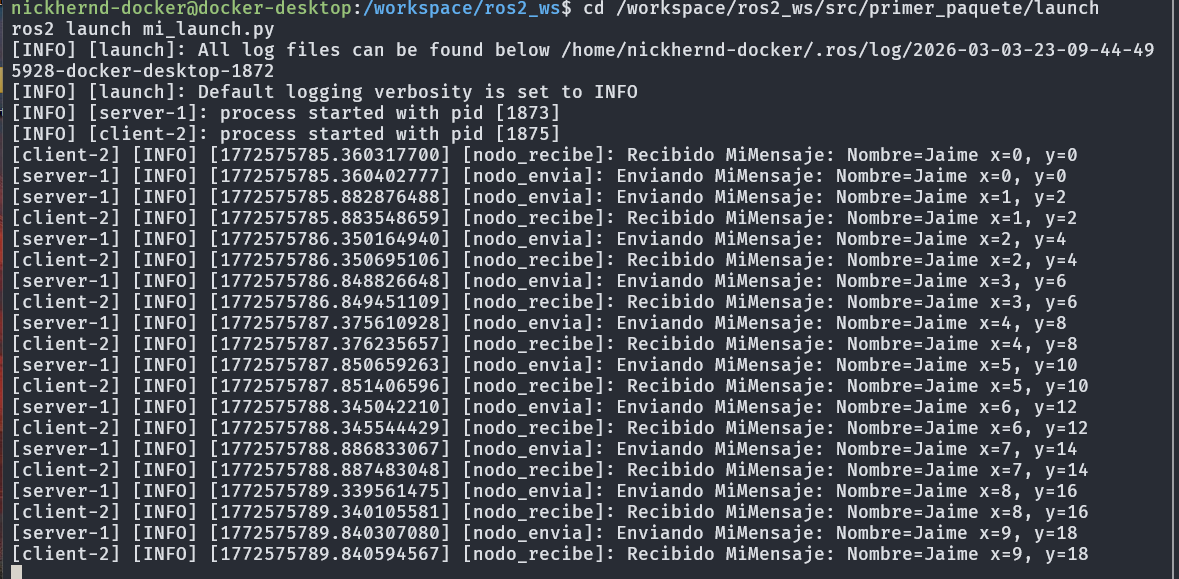
\includegraphics[width=0.85\textwidth]{parte3/imagenes/parte1.png}
  \caption{Nodos lanzados desde \texttt{mi\_launch.py} con sus nombres asignados.}
  \label{fig:p3_launch}
\end{figure}

%--------------------------------------------------------------
\section{Acciones}
%--------------------------------------------------------------

\subsection*{Pregunta 15}
\textit{¿Cómo podemos saber que se ha lanzado la acción correctamente? ¿Qué método permite saber que la acción ha finalizado exitosamente?}

La acción se ha lanzado correctamente cuando el servidor responde con \textit{goal accepted} y el cliente recibe el \texttt{goal\_id}. La acción finaliza exitosamente cuando el servidor ejecuta \texttt{goal\_handle.succeed()}, lo que dispara el callback \texttt{get\_result\_callback} en el cliente con el resultado final.

\begin{figure}[H]
  \centering
  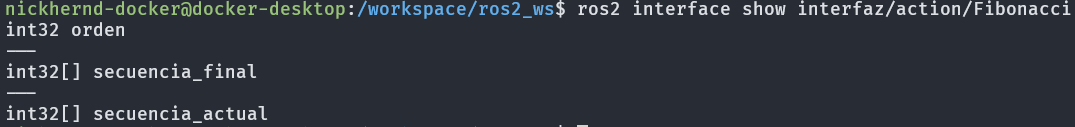
\includegraphics[width=0.85\textwidth]{parte3/imagenes/action_fibonacci.png}
  \caption{Servidor y cliente de la acción Fibonacci en ejecución.}
  \label{fig:p3_action}
\end{figure}

\subsection*{Pregunta 16}
\textit{Sin crear un nodo, ¿cómo lanzarías la acción Fibonacci? ¿Cómo observarías el resultado?}

Desde terminal, usando \texttt{ros2 action send\_goal} con el flag \texttt{--feedback} para ver el progreso:

\begin{lstlisting}[style=bash, caption={Lanzar la acción Fibonacci desde terminal.}]
ros2 action send_goal /fibonacci interfaz/action/Fibonacci \
    "{orden: 10}" --feedback
\end{lstlisting}

\begin{figure}[H]
  \centering
  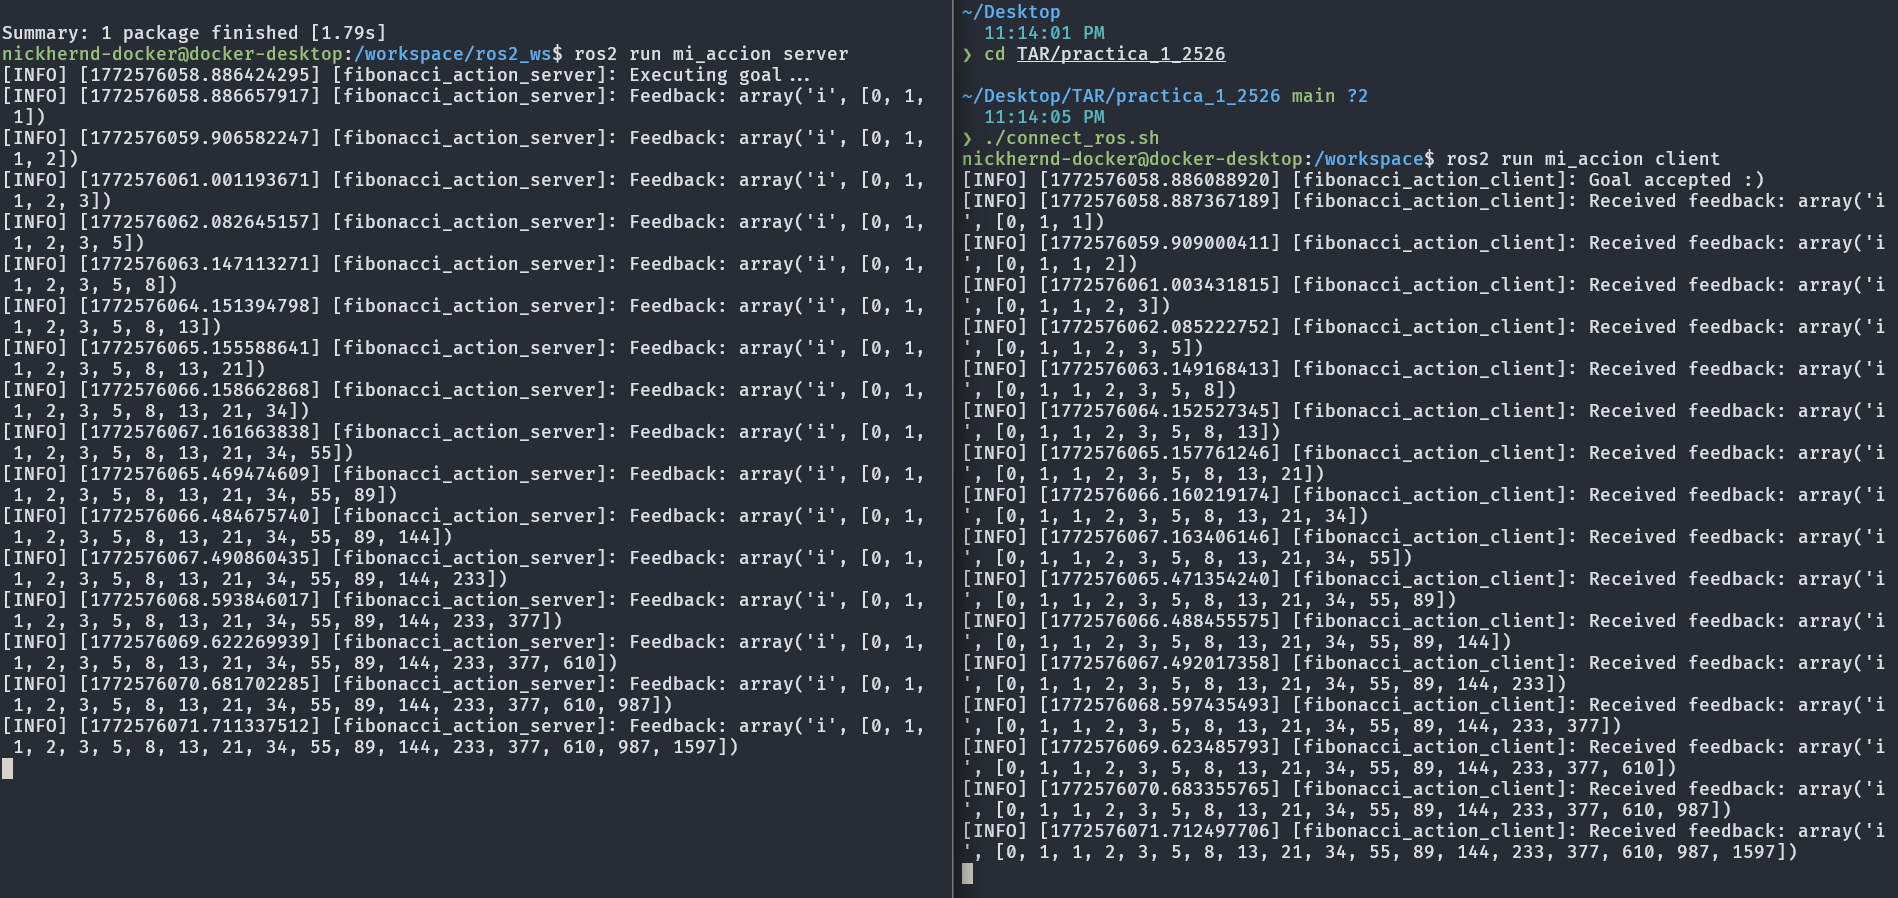
\includegraphics[width=0.85\textwidth]{parte3/imagenes/fib_accion_en_accion.png}
  \caption{Acción Fibonacci lanzada directamente desde terminal con feedback.}
  \label{fig:p3_action_terminal}
\end{figure}

\subsection*{Pregunta 17}
\textit{Si paramos el nodo a mitad de la ejecución, ¿se cancela la acción? ¿Se puede cancelar desde la terminal?}

Si se para el servidor (\texttt{Ctrl+C}), la acción no se cancela limpiamente: el cliente pierde la conexión y queda bloqueado sin recibir ni resultado ni cancelación. Sí se puede cancelar desde terminal mediante:
\begin{lstlisting}[style=bash]
ros2 action cancel <goal_uuid>
\end{lstlisting}
Siempre que el servidor tenga implementado un \texttt{cancel\_callback}.

%--------------------------------------------------------------
\section{Ejercicios}
%--------------------------------------------------------------

\subsection{Ejercicio 1: \texttt{launch\_ejercicio3.py}}

Fichero launch que lanza \texttt{nodopub\_ejercicio2} y \texttt{nodosub\_ejercicio2} con un argumento \texttt{numero} (por defecto 7) pasado como parámetro al publisher:

\begin{lstlisting}[style=python, caption={Argumento en launch\_ejercicio3.py.}]
numero_arg = DeclareLaunchArgument('numero', default_value='7')
Node(package='p2pkg', executable='nodopub_ejercicio2',
     parameters=[{'numero': LaunchConfiguration('numero')}])
\end{lstlisting}

\begin{figure}[H]
  \centering
  
\includegraphics[width=0.85\textwidth]{parte3/imagenes/ejercicio1.png}
  \caption{Ejecución de \texttt{launch\_ejercicio3.py} con argumento por defecto.}
  \label{fig:p3_ej1}
\end{figure}

\subsection{Ejercicio 2: \texttt{launch\_ejercicio4.py} con namespace y remapping}

Nota: listar nodos y topics

Los nodos se agrupan bajo el namespace \texttt{miGrupo} y se remapea el topic \texttt{/topic\_ejercicio2} a \texttt{/miGrupo/topic\_ejercicio2}:

\begin{lstlisting}[style=python, caption={Namespace y remapping en launch\_ejercicio4.py.}]
GroupAction([
    PushRosNamespace('miGrupo'),
    Node(..., remappings=[('/topic_ejercicio2',
                           '/miGrupo/topic_ejercicio2')]),
    ...
])
\end{lstlisting}

\begin{figure}[H]
  \centering
  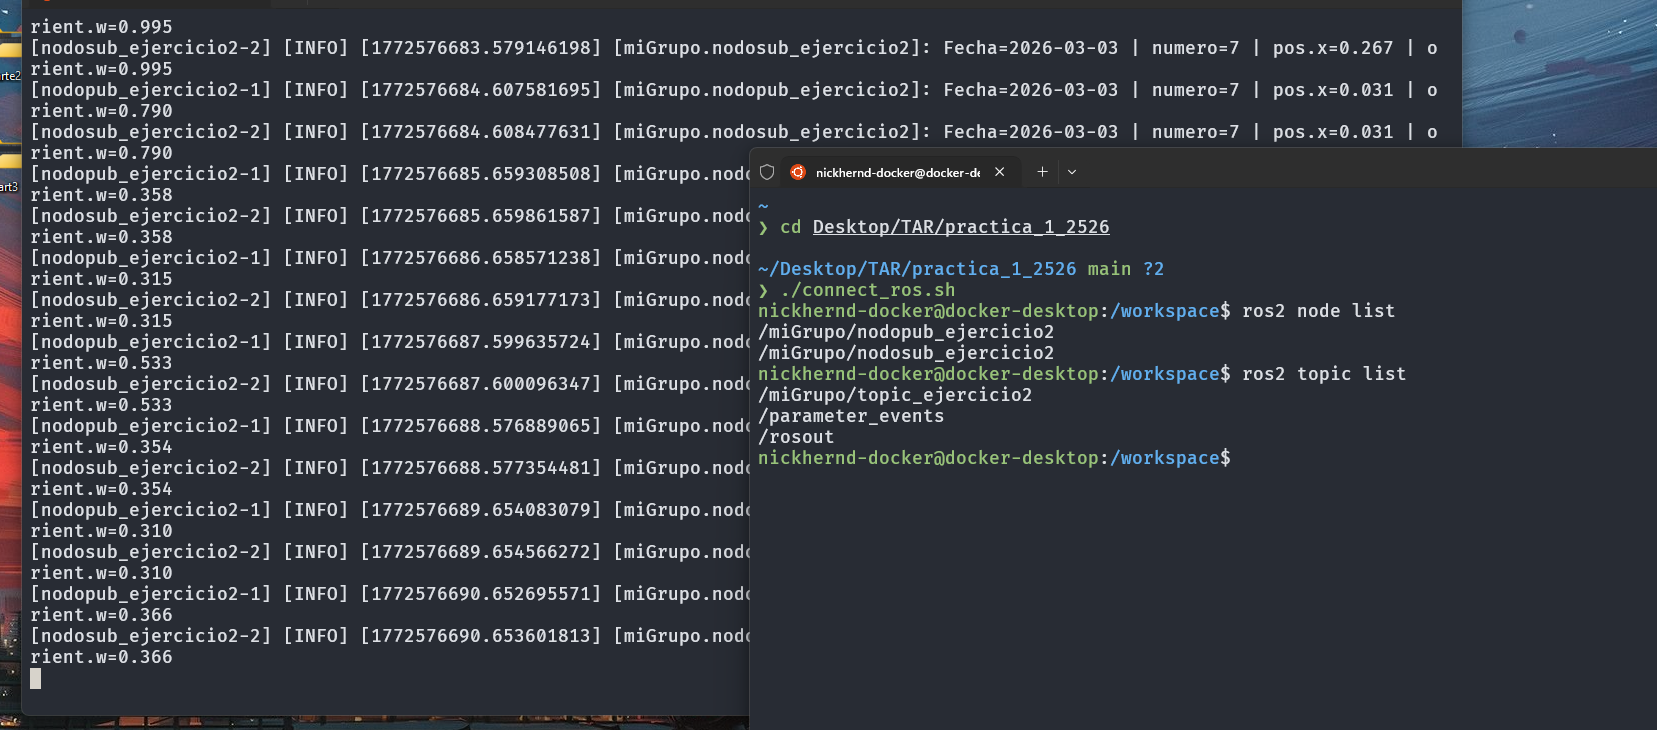
\includegraphics[width=0.85\textwidth]{parte3/imagenes/ejercicio2.png}
  \caption{\texttt{rqt\_graph} con nodos en el namespace \texttt{miGrupo}.}
  \label{fig:p3_ej2}
\end{figure}

\subsection{Ejercicio 3: Acción \texttt{EjFibonacci.action}}

Nueva acción con el mismo goal y result que \texttt{Fibonacci.action}, pero con feedback de tipo \texttt{float64}:

\begin{lstlisting}[caption={Definición de EjFibonacci.action.}]
int32 orden
---
int32[] secuencia_final
---
float64 feedback_value
\end{lstlisting}

\subsection{Ejercicio 4: Servidor \texttt{ejercicios\_fibServer.py}}

El servidor calcula la secuencia de Fibonacci y en cada iteración envía como feedback la raíz cuadrada de la media de la secuencia calculada hasta ese momento:

\begin{lstlisting}[style=python, caption={Cálculo del feedback en el servidor.}]
media = sum(secuencia) / len(secuencia)
feedback_msg.feedback_value = math.sqrt(media)
goal_handle.publish_feedback(feedback_msg)
\end{lstlisting}

\begin{figure}[H]
  \centering
  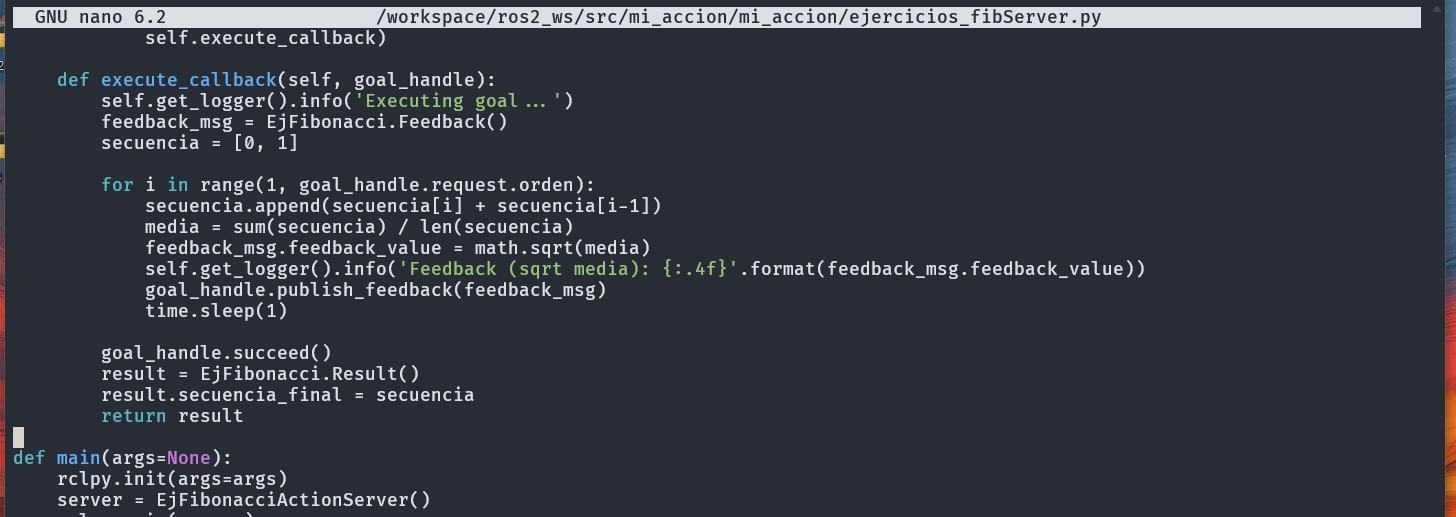
\includegraphics[width=0.85\textwidth]{parte3/imagenes/ejercicio4.png}
  \caption{Servidor \texttt{ejfibonacci\_action\_server} publicando feedback.}
  \label{fig:p3_ej4}
\end{figure}

\subsection{Ejercicio 5: Cliente \texttt{ejercicios\_fibClient.py}}

El cliente acepta el orden como argumento por línea de comandos y, mientras la acción está en curso, publica periódicamente el string \texttt{'en proceso'} en el topic \texttt{/estado\_accion}:

\begin{lstlisting}[style=python, caption={Publicación del estado mientras la acción está en curso.}]
def publish_estado(self):
    if self._in_progress:
        msg = String()
        msg.data = 'en proceso'
        self._publisher.publish(msg)
\end{lstlisting}

\begin{figure}[H]
  \centering
  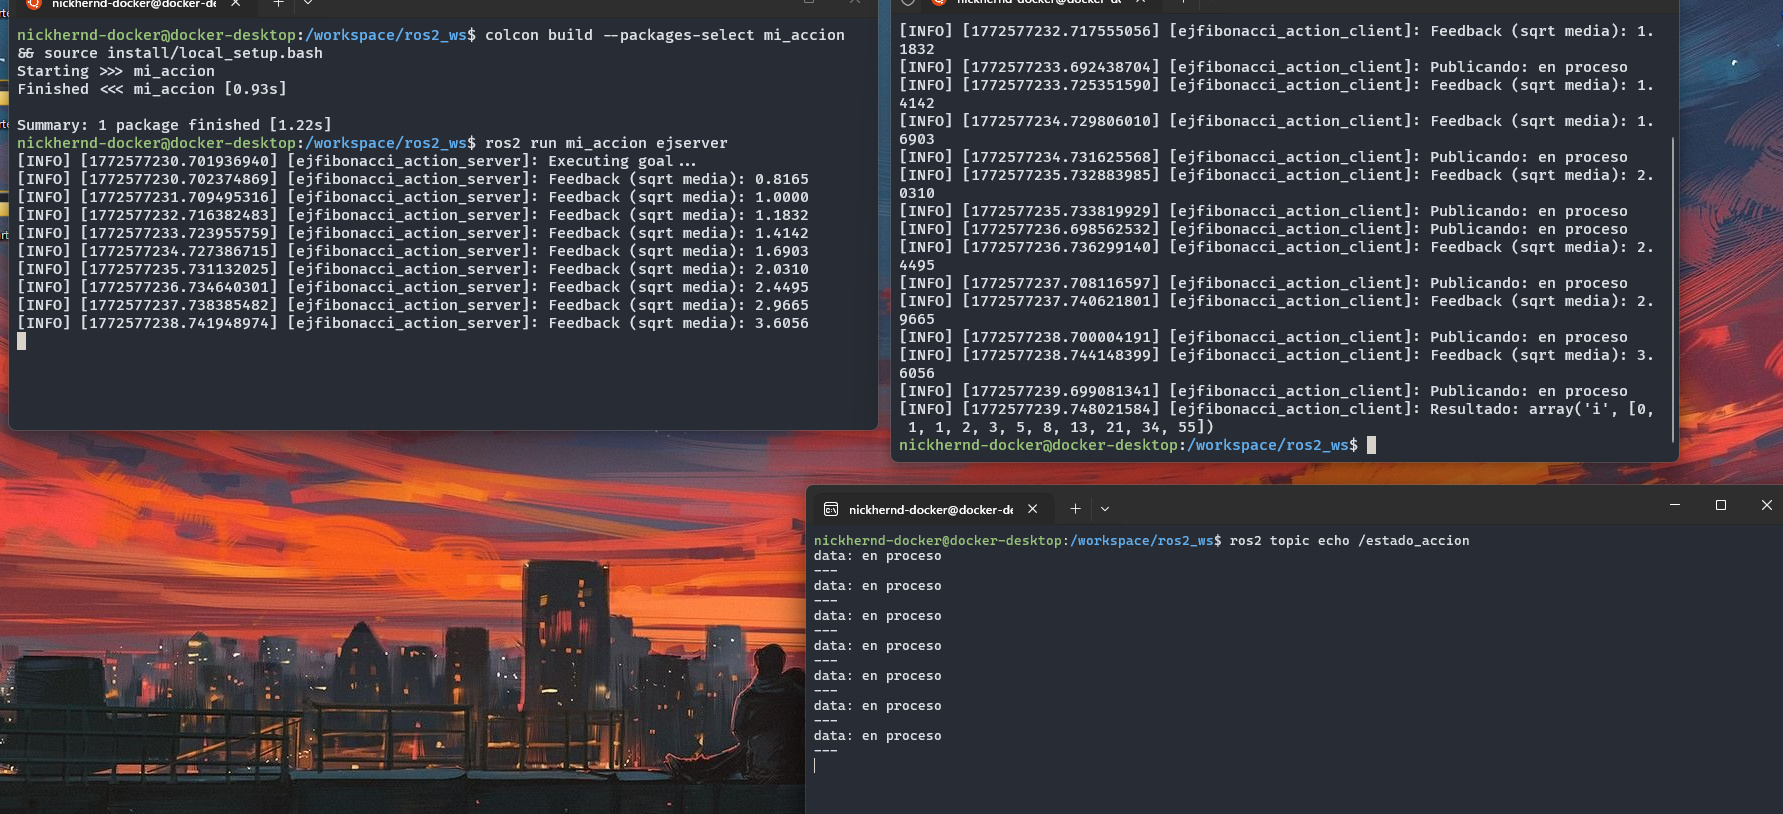
\includegraphics[width=0.85\textwidth]{parte3/imagenes/ejercicio5.png}
  \caption{Cliente recibiendo feedback y publicando estado en \texttt{/estado\_accion}.}
  \label{fig:p3_ej5}
\end{figure}

\subsection{Ejercicio 6: Servicio \texttt{service\_temp} (conversión de temperatura)}

Servicio que convierte entre Celsius y Fahrenheit según el campo \texttt{conversion\_type}:

\textbf{Interfaz} (\texttt{TempConversion.srv}):
\begin{lstlisting}[caption={Interfaz del servicio de temperatura.}]
float64 input_temp
string conversion_type   # "Cel_to_Far" o "Far_to_Cel"
---
float64 converted_temp
\end{lstlisting}

Las conversiones implementadas son:
\begin{itemize}
  \item \texttt{Cel\_to\_Far}: $T_F = T_C \times \frac{9}{5} + 32$
  \item \texttt{Far\_to\_Cel}: $T_C = (T_F - 32) \times \frac{5}{9}$
\end{itemize}

\begin{figure}[H]
  \centering
  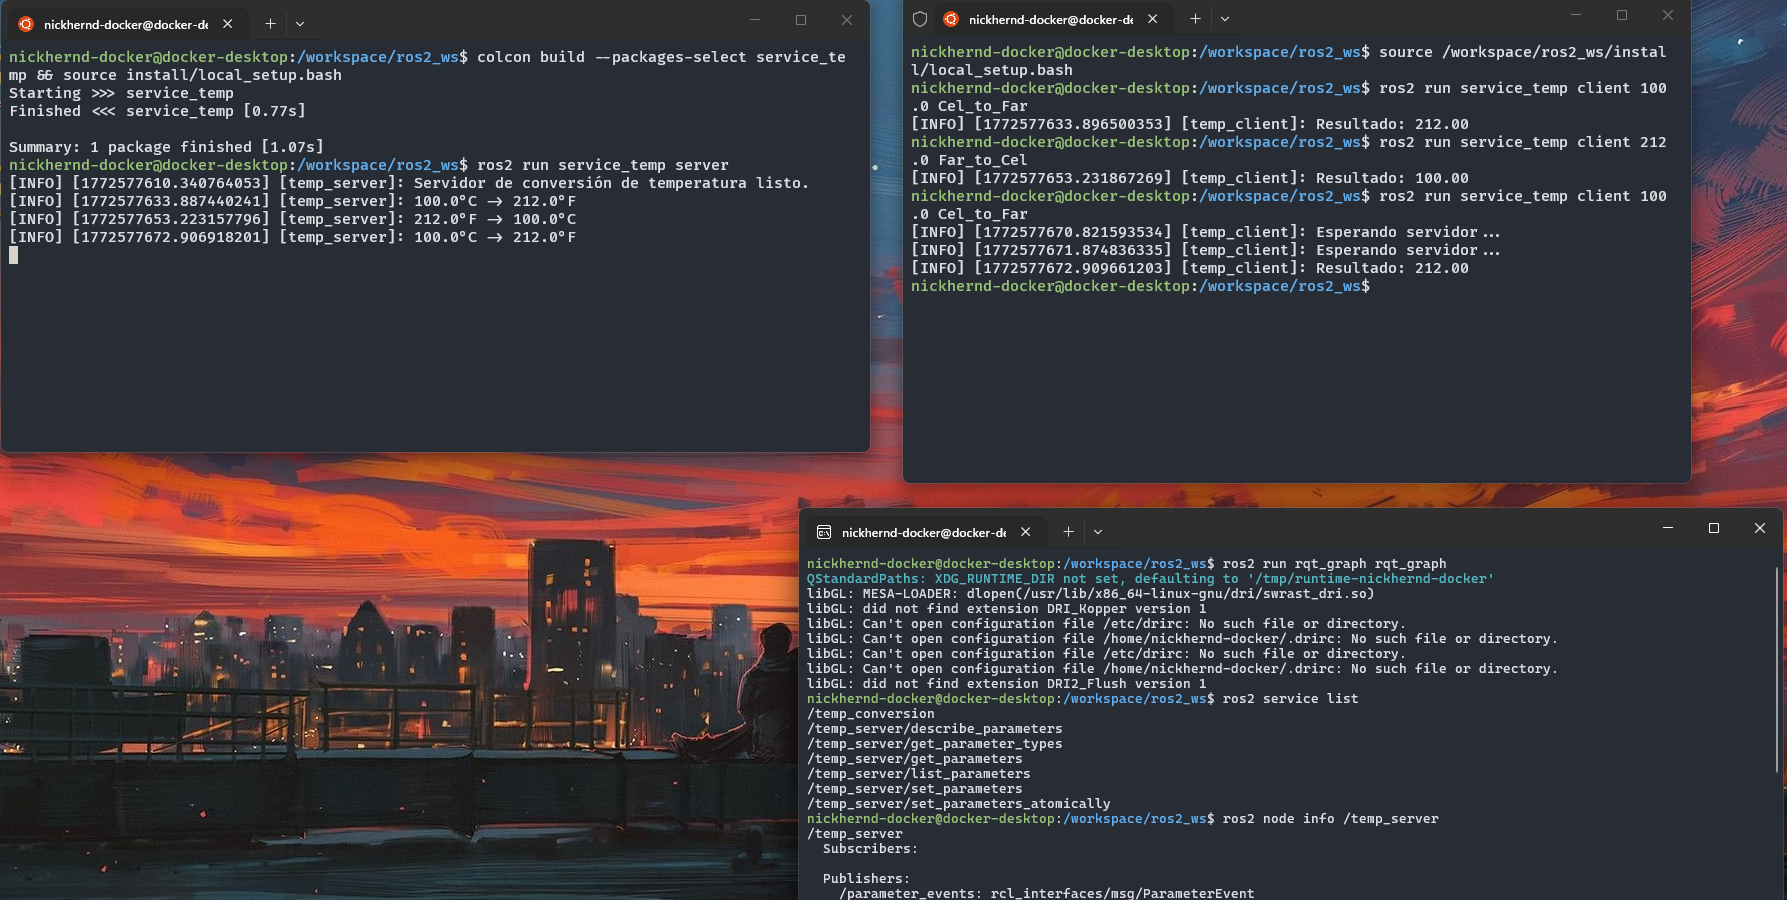
\includegraphics[width=0.85\textwidth]{parte3/imagenes/ejercicio6_finish.png}
  \caption{Ejecución del servicio de conversión de temperatura.}
  \label{fig:p3_ej6}
\end{figure}

\subsection{Ejercicio 7: Acción \texttt{battery\_act} (simulación de batería)}

Sistema que simula la descarga de la batería de un robot desde 100\% hasta un porcentaje objetivo.

\textbf{Interfaz} (\texttt{BatteryAction.action}):
\begin{lstlisting}[caption={Interfaz de la acción battery\_act.}]
int32 target_percentage
---
string warning
---
int32 current_percentage
\end{lstlisting}

El servidor (\texttt{battery\_charger}) decrementa la batería en 5\% cada segundo, publicando el nivel actual como feedback. Al alcanzar el objetivo, devuelve el mensaje de aviso \textit{``¡Batería baja, por favor cargue el robot!''}. Admite cancelación en cualquier momento gracias al \texttt{cancel\_callback}.

\begin{figure}[H]
  \centering
  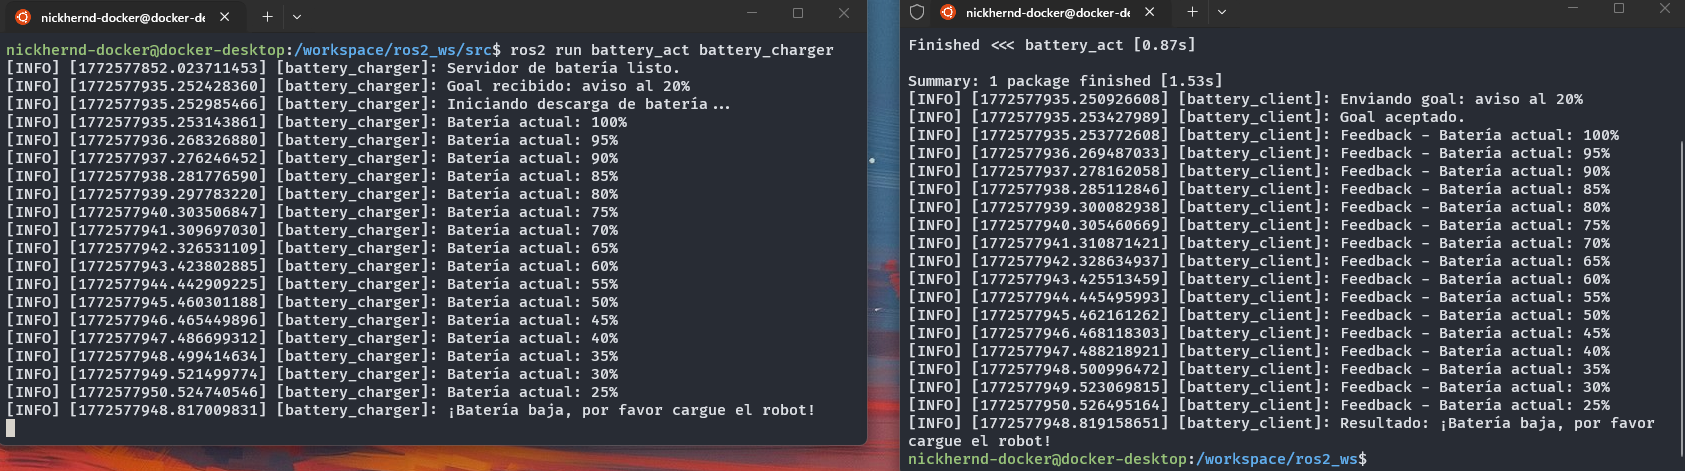
\includegraphics[width=0.85\textwidth]{parte3/imagenes/ejercicio7.png}
  \caption{Servidor \texttt{battery\_charger} y cliente \texttt{battery\_client} en ejecución.}
  \label{fig:p3_ej7}
\end{figure}


\end{document}
